
\section{Proyecto: Automatización Inteligente de Captura de Facturas}\label{sec:automatizacion-facturas}

\subsection{Eliminando Errores y Agilizando Procesos con IA}

\textbf{Problema Actual:}

En la mayoría de las maquiladoras en Ciudad Juárez, el procesamiento manual de facturas sigue siendo una tarea compleja y repetitiva que consume tiempo y recursos humanos. Imagina un equipo de \textbf{30 capturistas} dedicados exclusivamente a la revisión y captura manual de datos de facturas en diferentes formatos, ya sean PDF, imágenes o archivos XML. Este proceso es propenso a errores humanos y puede retrasar la cadena de suministros, afectando la producción y la relación con los proveedores.

El principal reto aquí es que, aunque la tecnología existe para automatizar este proceso, la mayoría de las maquilas siguen operando con métodos tradicionales, lo que genera ineficiencias que se traducen en costos más altos y tiempos de procesamiento más largos. En un entorno tan competitivo como el de las maquiladoras, esto puede significar una desventaja frente a empresas que ya han implementado tecnologías de automatización.

\textbf{Problema Hipotético:}

Una maquila que procesa \textbf{10,000 facturas mensuales} con diferentes formatos necesita optimizar su proceso para mejorar la eficiencia. Con \textbf{AutoFact 4.0}, el uso de \textbf{Large Language Models (LLM)} como \textbf{GPT-4} o \textbf{Gemini} permite a la maquila reducir significativamente el tiempo y los errores asociados al proceso manual. En lugar de tener un equipo de capturistas trabajando largas jornadas, \textbf{AutoFact 4.0} puede procesar la misma cantidad de facturas en cuestión de horas, utilizando su capacidad para leer, comprender y extraer datos de los diferentes formatos de facturas de manera automática.

\subsubsection{Objetivo del Proyecto}

Implementar \textbf{AutoFact 4.0}, un sistema basado en \textbf{LLM}, que automatice la captura y validación de facturas, utilizando reglas predefinidas de aduanas y normativas locales. Este sistema reducirá la necesidad de intervención humana, acelerará el proceso de facturación y garantizará el cumplimiento normativo con la aduana, optimizando la eficiencia y precisión del proceso.

\subsection{Implementación del Proyecto y Comunicación con Modelos LLM}

\textbf{AutoFact 4.0} no es solo un sistema que extrae información de las facturas; es una solución completa que integra \textbf{inteligencia artificial}, \textbf{procesamiento de lenguaje natural (NLP)} y \textbf{sistemas basados en reglas}. Al trabajar con diferentes formatos de archivos, como \textbf{PDFs} y \textbf{XML}, este sistema no solo identifica y extrae datos relevantes, sino que también los valida con base en \textbf{reglas aduaneras preestablecidas}.

\subsubsection{Paso 1: Recepción y Análisis de Facturas}

El primer paso es la recepción de las facturas. Estas llegan en diferentes formatos, ya sean PDF o XML. Aquí entra en juego una etapa clave de la implementación: la capacidad del sistema para \textbf{comunicarse entre diferentes formatos y los LLM}. Esto implica entrenar el modelo para que pueda interpretar estructuras variables de datos en los PDFs, que son generalmente más complejos, y los XML, que siguen un formato más estandarizado.

\begin{itemize}
    \item \textbf{PDFs}: Utilizando técnicas de reconocimiento óptico de caracteres (\textbf{OCR}), \textbf{AutoFact 4.0} convierte el contenido de las facturas en texto legible para el modelo LLM. A partir de ahí, el modelo extrae información clave como el monto total, el nombre del proveedor, la fecha de emisión y los detalles de los productos.
    \item \textbf{XMLs}: A diferencia de los PDFs, los archivos XML ya contienen la estructura de datos organizada, lo que permite a \textbf{AutoFact 4.0} extraer rápidamente los campos relevantes. El reto con los XML es su variabilidad en el formato dependiendo del proveedor, por lo que el sistema debe ser lo suficientemente flexible para adaptarse a estas diferencias.
\end{itemize}

\subsubsection{Paso 2: Validación Basada en Reglas Aduaneras}

Una vez que se extraen los datos, el siguiente paso es la \textbf{validación} de estos contra reglas aduaneras específicas. El sistema puede integrar una serie de \textbf{reglas predefinidas} que aseguran que los datos capturados cumplan con las regulaciones locales y normativas fiscales.

Por ejemplo, si una factura no incluye los datos necesarios del proveedor o los códigos correctos de los productos, \textbf{AutoFact 4.0} alertará al equipo para que se realicen las correcciones correspondientes antes de aprobar la factura.

\subsubsection{Paso 3: Optimización del Proceso y Reportes en Tiempo Real}

Además de procesar y validar las facturas, \textbf{AutoFact 4.0} también puede generar reportes en tiempo real que muestren el estado de cada factura, si ha sido aprobada, si está pendiente de revisión o si presenta alguna anomalía que necesita ser corregida. Este tipo de visibilidad es crucial para agilizar los tiempos de procesamiento y garantizar que no haya demoras que afecten las operaciones.

\subsection{Diagrama del Proceso}

\begin{figure}[H]
    \centering
    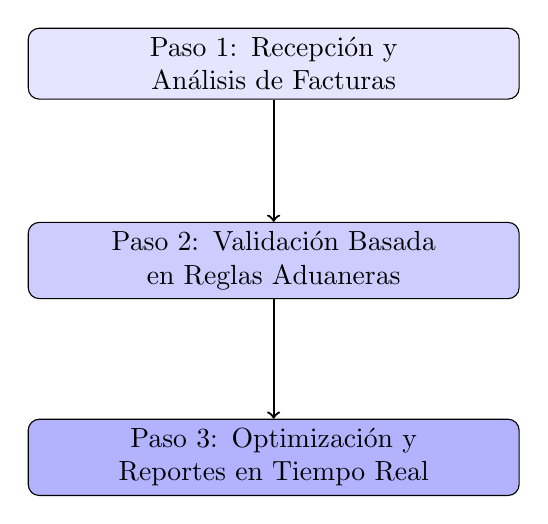
\begin{tikzpicture}
        \node[draw, fill=blue!10, text width=6cm, align=center, rounded corners] (p1) {Paso 1: Recepción y Análisis de Facturas};
        \node[below of=p1, node distance=2.5cm, draw, fill=blue!20, text width=6cm, align=center, rounded corners] (p2) {Paso 2: Validación Basada en Reglas Aduaneras};
        \node[below of=p2, node distance=2.5cm, draw, fill=blue!30, text width=6cm, align=center, rounded corners] (p3) {Paso 3: Optimización y Reportes en Tiempo Real};

        \draw[->, thick] (p1) -- (p2);
        \draw[->, thick] (p2) -- (p3);
    \end{tikzpicture}
    \caption{Diagrama de Proceso de AutoFact 4.0}
\end{figure}
\section{Ejemplo de Factura: Antes y Después del Procesamiento por AutoFact 4.0}

A continuación, se presenta un ejemplo de una factura en formato TXT desordenado antes de ser procesada, y luego el resultado de cómo sería la misma factura después de ser organizada y estructurada por **AutoFact 4.0**.

\begin{table}[H]
\centering
\caption{Comparación de Factura Desordenada y Ordenada por AutoFact 4.0}
\begin{tabularx}{\textwidth}{|X|X|}
\hline
\textbf{Factura Desordenada (Formato TXT/PDF)} & \textbf{Factura Ordenada (AutoFact 4.0)} \\ \hline
\texttt{N\#Factura:  202309123   \hspace{1.2cm}   \\
Proveedor: ACME Corp\\
Articulos:\\
20230912\hspace{0.5cm} Cantidad: 20 \hspace{0.8cm} Producto: Componentes\\
Sub-Total: \$5,000.00\\
IVA: \$800.00 \hspace{2cm}  (16\%)\\
Total:   \$5,800.00   Fecha: 12-09-2023\\
Receptor: Maquila XYZ\\
Direccion:\\ 123 Calle Industrial,\\ Ciudad Juárez, Chihuahua, 32000\\} 
& 
\textbf{N\#Factura:} 202309123 \\
\textbf{Fecha de Emisión:} 12-09-2023 \\
\textbf{Proveedor:} ACME Corp \\
\textbf{Productos:} \\
- \textbf{Descripción:} Componentes \\
- \textbf{Cantidad:} 20 \\
\textbf{Sub-Total:} \$5,000.00 \\
\textbf{IVA (16\%):} \$800.00 \\
\textbf{Total:} \$5,800.00 \\
\textbf{Receptor:} Maquila XYZ \\
\textbf{Dirección de Entrega:} \\
123 Calle Industrial, Ciudad Juárez, Chihuahua, 32000 \\ \hline
\end{tabularx}
\end{table}

\textbf{Descripción del Proceso:}

En la columna izquierda, tenemos un ejemplo de cómo llega la factura en un formato desordenado, ya sea en TXT o PDF, con datos distribuidos de manera inconsistente. Después de que el sistema **AutoFact 4.0** procesa la información, se organiza de forma clara y estructurada, como se muestra en la columna derecha. El sistema es capaz de identificar y extraer automáticamente los campos importantes como el número de factura, el proveedor, la cantidad de productos, el total y otros detalles relevantes, lo que facilita la revisión y validación de la factura.

\subsection{Ventajas de AutoFact 4.0}

\begin{itemize}
    \item \textbf{Reducción de la Intervención Humana}: El número de capturistas se reduce drásticamente. Con AutoFact 4.0, en lugar de 30 capturistas, solo se necesita un equipo pequeño que supervise el sistema.
    \item \textbf{Integración con Normas Aduaneras}: AutoFact 4.0 verifica automáticamente que cada factura cumpla con las normativas vigentes, evitando problemas legales.
    \item \textbf{Mayor Rapidez y Precisión}: Los LLM permiten procesar miles de facturas en minutos con una alta precisión, minimizando errores humanos.
    \item \textbf{Escalabilidad}: El sistema se adapta a un mayor volumen de facturas sin requerir una expansión significativa del equipo humano.
\end{itemize}

\subsection{Consideraciones Técnicas}

La implementación de AutoFact 4.0 requerirá un esfuerzo técnico significativo debido a la integración con los formatos de facturas y la personalización de las reglas aduaneras. Algunos pasos clave incluyen:

\begin{itemize}
    \item Capacitación del equipo de TI en el manejo de LLMs.
    \item Ajuste de las reglas aduaneras para adaptarse a las normativas específicas de cada maquila.
    \item Evaluaciones periódicas para asegurar que el sistema funcione correctamente.
\end{itemize}

\subsection{Comparación Antes y Después de Implementar AutoFact 4.0}

\begin{table}[H]
\centering
\caption{Comparación Antes y Después de Implementar AutoFact 4.0}
\begin{tabular}{|l|c|c|}
\hline
\textbf{Métrica} & \textbf{Antes de AutoFact 4.0} & \textbf{Después de AutoFact 4.0} \\ \hline
Tiempo de procesamiento por factura & 15 minutos por factura & 2 minutos por factura \\ \hline
Errores de captura & 5-10\% & Menos del 1\% \\ \hline
Cantidad de capturistas & 30 capturistas & 5 supervisores \\ \hline
Costo estimado por factura & \$0.10 USD & \$0.02 USD \\ \hline
Facturas procesadas al mes & 10,000 facturas & 10,000 facturas (con posibilidad de escalar) \\ \hline
\end{tabular}
\end{table}

\subsubsection{Costo Estimado del Proyecto}

El costo estimado por factura utilizando \textbf{AutoFact 4.0} se reducirá de \$0.10 USD a \$0.02 USD, lo que representa una reducción significativa de costos. Además, se reducirá el tiempo de procesamiento y se incrementará la precisión de los datos, mejorando la eficiencia general del proceso de captura de facturas en la maquila.

